\section{Plateau-Cap Spring Lag: Modeled Soil Null and Guild Evidence}
\label{sec:plateau_guild}

At the upper margin of the escarpment, spring green-up steps sharply later onto the flat sandstone tableland (\cref{fig:hopkins_decomp}a). Stratified comparisons show this lag does not stem simply from crossing the 547~m limestone--sandstone lithologic contact: holding steep slope constant ($>10^\circ$, 507~m to 566~m) in \texttt{SCS+C} NDRE shifts spring by $+3.11 \pm 0.53$~d (SE, $n=7$~yr) and autumn by $-3.34 \pm 0.41$~d (SE; \texttt{HLS v2.0} NDRE $+3.12$ / $-3.05$~d). Above the sandstone contact ($\ge 550$~m), flat plateau benches ($\le 8^\circ$, mean elevation 575.4~m) lag adjacent steep rocky rims ($>10^\circ$, mean 566.8~m) by $+3.53$~d across just $+8.62$~m of elevation ($+3.31$~d inside \texttt{EVT 3317} alone). Flat and steep plateau canopies share nearly identical winter NDVI ($0.416$ vs.\ $0.427$), ruling out evergreen understory contamination.

\begin{figure}[t]
\centering
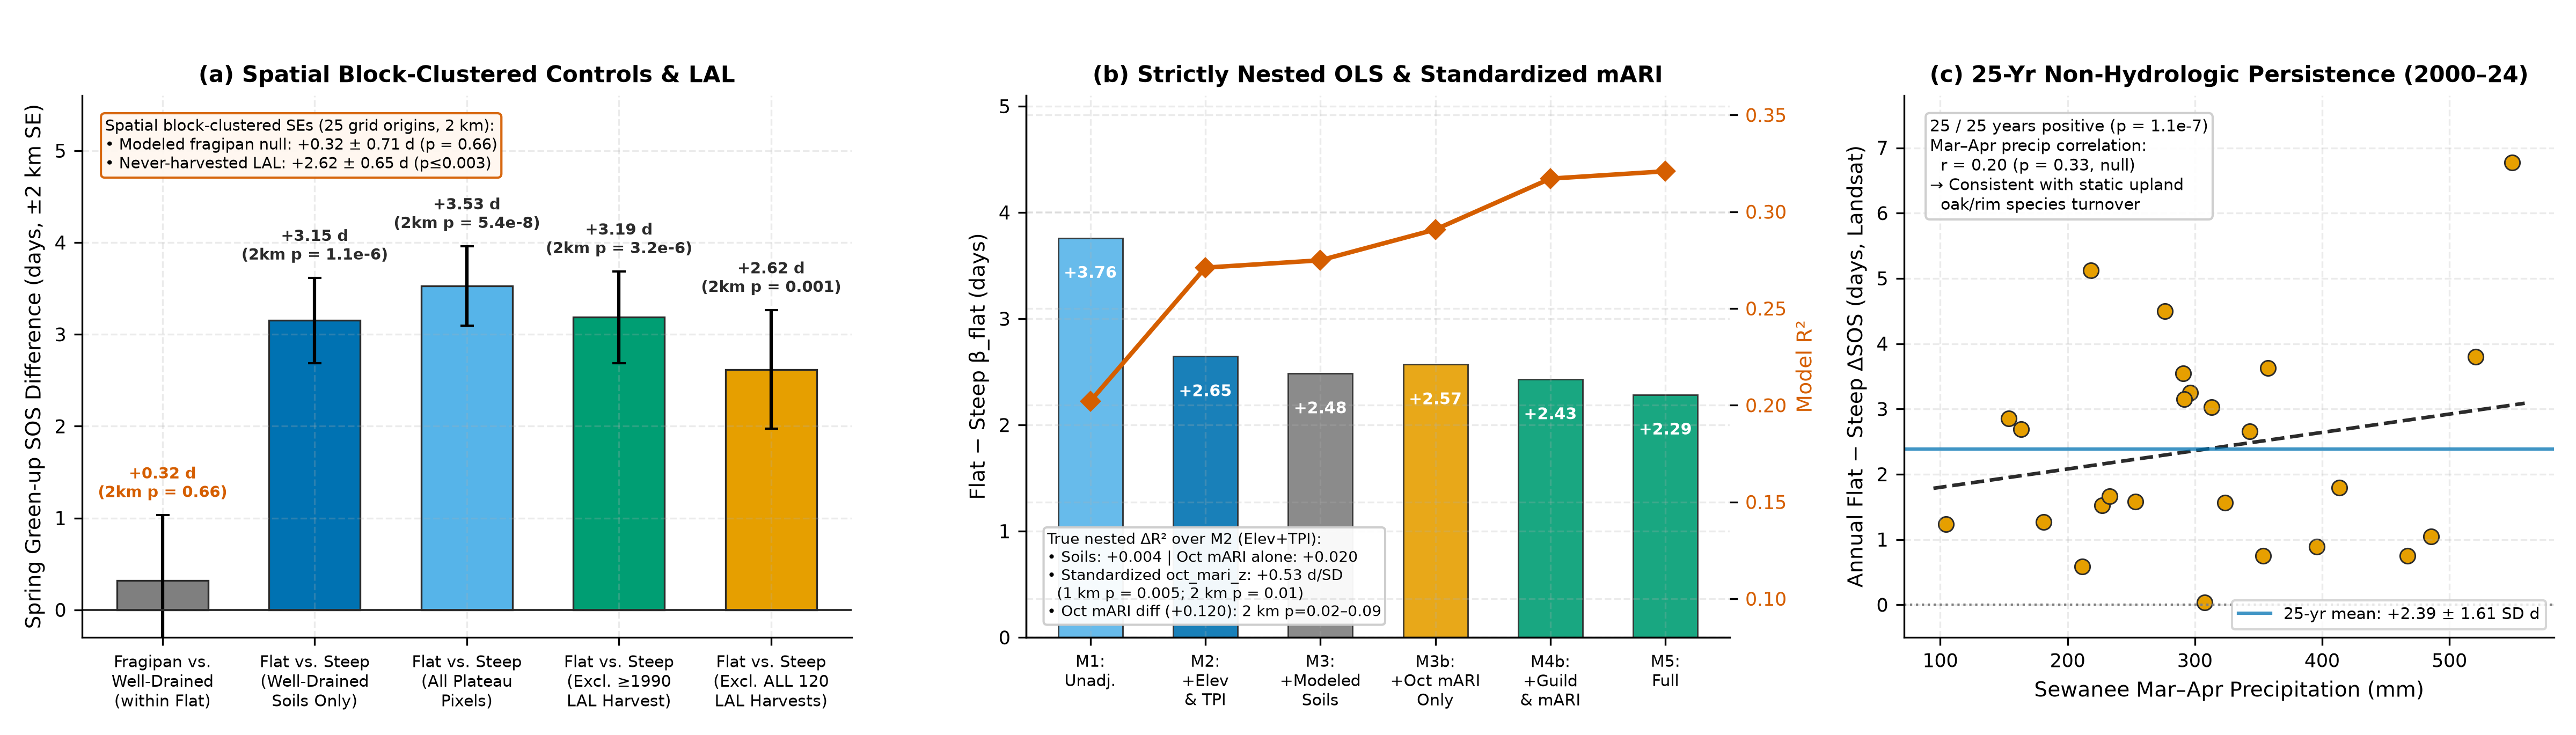
\includegraphics[width=\linewidth]{figures/fig6.png}
\caption{\textbf{Spatial block-clustered tests rule out modeled fragipan inertia and are consistent with plateau-cap guild turnover.} (a)~Multi-origin 2~km spatial block-clustered estimates (mean $\pm$ median 2~km SE across 25 grid origins): within-flat fragipan shows zero delay ($+0.32 \pm 0.71$~d, $p=0.66$), whereas well-drained ($+3.15$~d) and never-harvested LAL stands ($+2.62$~d) remain significant ($p \le 0.0032$). (b)~Strictly nested OLS shows modeled soils add $\Delta R^2=+0.004$, while standardized October \texttt{mARI} enters at $+0.53$~d/SD ($\Delta R^2=+0.020$ alone). (c)~Flat stands lag in 25/25 Landsat years ($+2.39 \pm 1.61$~d SD) with no spring precipitation trend ($r=0.20, p=0.33$).}
\label{fig:plateau_guild}
\end{figure}

Two mechanisms competed under internal criterion P5: (i)~\emph{pedological thermal inertia}, wherein dense subsurface fragipans on flat benches perch cold spring rainwater and delay root warming, and (ii)~\emph{upland oak guild turnover}, wherein level fire-prone sandstone uplands favor late-leafing ring-porous oaks and hickories (\emph{Quercus coccinea}, \emph{Q.\ alba}, \emph{Q.\ montana}) over earlier-flushing mesophytes (\emph{Liriodendron tulipifera}, \emph{Acer rubrum}) sheltered along steep rocky rims. Because 30~m pixels are spatially autocorrelated, we evaluate all plateau-cap contrasts using CR1 spatial block-clustered standard errors across 25 multi-origin grid alignments at both 1~km and 2~km block sizes rather than unclustered pixel $p$-values (\cref{fig:plateau_guild}a).

Modeled soil inertia is falsified across every check. Within the flat plateau cap ($n=700$~pixels), \texttt{gNATSGO}/SSURGO fragipan or poorly drained soils differ from well-drained Hartsells and Ramsey soils by only $+0.32$~d (1~km median SE $= 0.76$~d, $p=0.64$--$0.74$; 2~km median SE $= 0.71$~d, $p=0.55$--$0.74$, 0\% of grid origins $<0.05$). Adding 30~m \texttt{POLARIS} hydraulic conductivity, clay, and bulk-density layers \citep{chaney2019} plus \texttt{gNATSGO} fragipan indicators to an elevation-and-TPI baseline (M2) raises $R^2$ by only $+0.0038$ ($0.271$ to $0.275$; \cref{fig:plateau_guild}b). Over 25 Landsat years (2000--2024), flat benches lag steep rims in 25/25 years ($+2.39 \pm 1.61$~d SD, one-sample $p=1.1 \times 10^{-7}$), with no correlation to March--April precipitation ($r=0.20, p=0.33$; \cref{fig:plateau_guild}c). Because \texttt{POLARIS} and \texttt{gNATSGO} are smoothed modeled soil products, this null falsifies mapped fragipan inertia while leaving unmapped fine-scale edaphic effects possible.

By contrast, four lines of evidence are \emph{consistent with} upland oak guild turnover. First, holding mapped well-drained soils constant ($n=1{,}199$), flat benches still lag steep rims by $+3.15$~d across all 25 spatial block origins (1~km median SE $= 0.39$~d, $p \le 4.5 \times 10^{-9}$; 2~km median SE $= 0.47$~d, $p \le 7.1 \times 10^{-6}$). Second, masking all 120 public Sewanee LAL harvest polygons reduces the raw lag by $\sim 0.9$~d (reflecting silvicultural history) yet leaves $+2.62$~d on never-harvested stands ($n=435$; 1~km median SE $= 0.56$~d, $p \le 0.00063$; 2~km median SE $= 0.65$~d, $p \le 0.0032$, 100\% of origins $<0.01$). Third, the flat-vs-steep lag replicates across all three regional escarpment sites with $\ge 550$~m plateau caps in our archived four-cove dataset: Sewanee ($+2.66$~d, $n=230/38$), Fiery Gizzard ($+2.39$~d, $n=244/15$), and Savage Gulf ($+4.09$~d, $n=218/31$). Fourth, flat plateau canopies exhibit higher October Modified Anthocyanin Reflectance Index (\texttt{mARI}, \citealp{gitelson2001}; $+0.120$), characteristic of red-foliage upland oaks: in strictly nested regressions, standardized \texttt{oct\_mari\_z} enters at $+0.53$~d per SD (1~km median SE $= 0.18$~d, $p=0.0011$--$0.015$; 2~km median SE $= 0.19$~d, $p=0.0015$--$0.065$, 84\% of origins $<0.05$) and adds true single-variable $\Delta R^2=+0.020$ over M2 (full guild plus \texttt{mARI} adds $+0.046$). Notably, the unadjusted flat-vs-steep \texttt{oct\_mari} difference ($+0.120$) is grid-alignment-sensitive at 2~km clustering ($p=0.017$--$0.094$, 36\% of origins $<0.05$; 1~km $p=0.012$--$0.036$). Because no ground species tallies were collected, we interpret these patterns as consistent with---rather than direct plot-level proof of---upland oak guild turnover.

\begin{table}[t]
\centering
\begin{threeparttable}
\caption{\textbf{Complete internal decision-criteria ledger (H1--H7), reporting exact verdicts including partial passes and falsified predictions.}}
\label{tab:hypothesis_ledger}
\small
\begin{tabularx}{\linewidth}{@{} l l >{\raggedright\arraybackslash}X @{}}
\toprule
ID & Status & Key Quantitative Evidence (All $\pm$ Labeled) \\
\midrule
H1 & \textbf{Supported} & MODIS 50\% \texttt{MidGreenup\_1} $= 3.19 \pm 0.17$~d/100~m SE (Hopkins $= 3.28$, trend $p=0.86$); 3-factor decomposition attributes $-0.80$~d/100~m to 50\% vs.\ 15\% metric ($+0.01$ QA/NLCD); Landsat 2013 step non-identifiable ($p=0.91$). \\
H2 & \textbf{Partial/Fail} & \texttt{SCS+C} retains 99.6\% SOS / 98.1\% EOS; Signal~B aspect-invariant ($+2.30$ to $+3.32$~d) and survives unlogged stands ($+2.62$~d, 2~km $p \le 0.0032$). Internal gate P2 recorded as \texttt{PARTIAL\_OR\_FAIL}. \\
H3 & \textbf{Partial Pass} & 11 pairs (NDRE): relief-adj.\ CR1 $\Delta\text{GSL}=-9.07 \pm 1.81$~d SE ($p=0.00053$); rim-free $\Delta z$-adj.\ $-8.75 \pm 1.85$~d SE ($p=0.0011$); persists in \texttt{EVT 3317} ($-11.2$~d) and \texttt{3321} ($-6.8$~d); binary closure partial $R^2=54.4\%$ over relief (0--22~m unobserved). P1 \texttt{PARTIAL\_PASS}. \\
H4 & \textbf{Supported$^*$} & 52 cloud-leak-filtered \texttt{ECOSTRESS} nights (8 \texttt{v002} leaks dropped): spring $-0.96 \pm 0.22^\circ$C SE ($p=0.00042$), autumn $-1.49 \pm 0.29^\circ$C SE ($p=1.1{\times}10^{-5}$); Lost Cove wind collapse over 2.5--3.0~m/s ($p=0.0041$); 7/7 \texttt{16SED} coves individually $p \le 0.018$ ($-1.09 \pm 0.22^\circ$C SE). $^*$Leak-adjusted swath Manski bounds span 0. \\
H5 & \textbf{Split} & Modeled fragipan inertia \textbf{falsified} ($+0.32 \pm 0.71$~d 2~km SE, $p=0.66$; 25-yr precip $r=0.20$). Consistent with oak guild turnover ($+3.15$~d well-drained, 25/25~yr $+2.39$~d, \texttt{oct\_mari\_z} $+0.53$~d/SD, 2~km \texttt{mARI} diff grid-sensitive). \\
H6 & \textbf{Falsified} & Internal S2 April-freeze vertical decoupling failed ($r=-0.20, p=0.66$; freeze vs.\ mild $p=0.76$). HLS $r=-0.79$ and post-DOY-100 split ($p=0.025$) are exploratory only. \\
H7 & \textbf{Falsified} & 25-yr 4-cove \texttt{CalmOctFreeze} panel showed \emph{opposite} sign ($\beta=+1.18 \pm 0.53$~d/SD SE, $p=0.035$) as hard regional freezes ($\beta=+1.85$~d/SD) affect rims and floors together. \\
\bottomrule
\end{tabularx}
\end{threeparttable}
\end{table}
